\documentclass[conference]{IEEEtran}
\IEEEoverridecommandlockouts

\usepackage{cite}
\usepackage{amsmath,amssymb,amsfonts}
\usepackage{algorithmic}
\usepackage{graphicx}
\usepackage{textcomp}
\usepackage{xcolor}
\usepackage{booktabs}
\usepackage{tikz}
\usetikzlibrary{shapes.geometric, arrows}

\def\BibTeX{{\rm B\kern-.05em{\sc i\kern-.025em b}\kern-.08em
    T\kern-.1667em\lower.7ex\hbox{E}\kern-.125emX}}

\setlength{\parindent}{0pt}
\setlength{\parskip}{4pt}

\begin{document}

\title{Workload-Aware Adaptive Growth for Dynamic Arrays}



\maketitle

\begin{abstract}
Dynamic arrays are fundamental structures in modern software for fast random access and dynamic memory allocation. Conventional implementations resize arrays using fixed growth factors, compromising between memory utilization and resizing overhead. Although recent studies explore alternative array organizations to improve memory efficiency, their resizing strategies remain workload-independent, showing limited adaptability. This paper proposes a workload-aware growth strategy that adapts array expansion using resize history, current capacity, and insertion velocity. A hybrid logarithmic--harmonic growth function is parameterized using Gaussian-process Bayesian optimization and evaluated against fixed 1.5$\times$ and 2.0$\times$ growth policies and the CPython list policy across seven insertion patterns and workloads of $10^4$--$10^7$ elements. Under the $10^7$-element mixed workload, the proposed strategy reduced unused capacity from 4.63\% for fixed doubling to 0.42\% while retaining the same 20 reallocations and 10.49 million copied elements. Across the evaluated workloads, adaptive growth generally reduced memory waste without substantially increasing resizing overhead. These results indicate that workload-responsive capacity growth can improve the memory--reallocation trade-off of contiguous dynamic arrays, although evaluation in native container implementations remains necessary.
\end{abstract}

\begin{IEEEkeywords}
Dynamic arrays, Adaptive resizing, Workload-aware growth, Memory allocation, Dynamic memory management, Bayesian optimization
\end{IEEEkeywords}

\section{Introduction}
In modern software engineering, dynamic arrays are among the most widely used sequential containers, providing $O(1)$ constant-time random access and flexibility to adjust capacity during runtime \cite{cormen_algorithms}. Containers such as C++ \texttt{std::vector}, Java \texttt{ArrayList}, and CPython \texttt{list} maintain elements contiguously in physical memory to maximize cache locality and prefetching efficiency. However, when the allocated capacity of an array is exhausted, runtime must allocate a larger memory block from operating system allocator, copy all existing elements into the new block, and release the old memory block.

To guarantee that the amortized time complexity of element insertion remains $O(1)$, standard high-level implementations use geometric growth policies \cite{optimal_resizable}. Dynamic-array growth policies are implementation-dependent: Java \texttt{ArrayList} and MSVC STL \texttt{std::vector} use approximately $1.5\times$ growth \cite{java_data_structures}, GCC libstdc++ implements fixed doubling ($2.0\times$), and CPython \texttt{list} implements a bit-shifting overallocation rule ($\text{new\_allocated} = \text{newsize} + (\text{newsize} \gg 3) + (\text{newsize} < 9 \,\,?\,\, 3 : 6)$) in \texttt{listobject.c} \cite{python_list_impl}.

Although constant geometric growth factors are simple to implement, they present a rigid trade-off between memory waste (spatial cost) and resizing overhead (temporal cost). A fixed doubling factor ($2.0\times$) minimizes the number of reallocations and element copies, but it can result in up to 50\% memory waste if array ceases growing shortly after a reallocation. Conversely, conservative shifting policies (such as CPython's overallocation rule) minimize unused capacity but trigger frequent reallocations, leading to high CPU and element-copying overhead for large datasets. Furthermore, these static policies are completely workload-independent, reacting identically to slow steady streams and sudden high-velocity bursts of data insertions.

This paper addresses these limitations by introducing a workload-aware, adaptive dynamic array growth algorithm. The proposed framework transitions from static growth factors to dynamic function $g(k, v, C_{\text{old}})$, which continuously adjusts growth based on the array's resize history ($k$), current capacity ($C_{\text{old}}$), and real-time insertion velocity ($v$).

The contributions of this study are as follows:
\begin{enumerate}
    \item A workload-aware dynamic-array growth rule that incorporates capacity ($C_{\text{old}}$), resize history ($k$), and insertion velocity ($v$);
    \item A Bayesian-optimization procedure for calibrating adaptive growth parameters under a joint memory and resizing cost objective; and
    \item An empirical evaluation across multiple insertion patterns and workload scales against fixed geometric and CPython resizing policies.
\end{enumerate}

\section{Related Work}

\subsection{Resizable Array Growth Strategies}
The theoretical study of resizable arrays has long history rooted in amortized analysis and data structure design. Cormen et al. \cite{cormen_algorithms} establish classical proof that a geometric growth factor guarantees $O(1)$ amortized insertion, provided the factor is strictly greater than 1. Brodnik et al. \cite{optimal_resizable} extended this by proving that arrays can be implemented with both $O(1)$ worst-case access time and $O(\sqrt{n})$ wasted space simultaneously, using a two-tier block indexing scheme over fixed-size blocks. Tarjan and Zwick \cite{time_space_complexity} further sharpened these bounds, characterizing fundamental time--space trade-offs for dynamic sequences and demonstrating that no scheme can simultaneously achieve $O(1)$ amortized cost, optimal space, and worst-case guarantees. Rosenberg \cite{allocating_storage, managing_storage} examined allocation strategies for extendible arrays, introducing notions of storage efficiency that remain relevant to modern container design.

A parallel research direction addresses the resizing problem by abandoning the requirement that array elements occupy a single contiguous memory block. Hoogerwoord \cite{logarithmic_arrays} proposed a logarithmic implementation in which array is partitioned into exponentially sized segments, avoiding wholesale copying at the cost of slightly degraded access patterns. Bille et al. \cite{resizable_optimal_time_space} demonstrated fast dynamic arrays that achieve $O(1)$ worst-case push and pop operations with optimal space, again relying on segmented layouts. Katajainen \cite{fast_array} studied worst-case-efficient dynamic arrays and showed that practical implementations could maintain near-theoretical guarantees under adversarial sequences. Sartor et al. \cite{z_rays} introduced Z-rays, a hybrid scheme that decomposes arrays into contiguous sub-arrays having increasing sizes to balance access speed with reallocation economics. Dechev et al. \cite{lock_free_vector} studied lock-free dynamically resizable arrays for concurrent settings, and Dietz \cite{persistent_arrays} examined fully persistent arrays.

Also, dynamic memory allocation literature provides additional context for container resizing. Wilson et al. \cite{dynamic_storage_allocation} surveyed dynamic storage managers, documenting how fragmentation and policy choices in \texttt{malloc}/\texttt{free} implementations affect real-world performance. Berger et al. \cite{reconsidering_custom_allocation, hoard_allocator} analyzed custom and multithreaded allocation scalability, and Frigo et al. \cite{frigo_cache_oblivious} contributed the cache-oblivious model. The approaches reviewed here primarily rely on predefined growth or layout policies rather than adapting contiguous-array growth directly to observed insertion intensity.

\subsection{Adaptive Parameter Optimization}
In systems tuning, Snoek et al. \cite{practical_bayesian_opt} introduced the application of Gaussian Process Bayesian Optimization (GP-BO) to hyperparameter search, demonstrating that GP surrogate models can efficiently navigate complex parameter spaces with minimal function evaluations. Shahriari et al. \cite{bayesian_opt_review} reviewed Bayesian optimization methods, surrogate models, and acquisition functions. Jones et al. \cite{jones_ego} formulated the Efficient Global Optimization (EGO) framework, upon which modern GP-BO libraries such as scikit-optimize \cite{scikit_optimize} are built. While GP-BO has been applied to compiler flags and database knob tuning, its application to calibrating container growth models under multi-objective trade-offs represents an effective approach.

\section{Methodology}

\subsection{Growth Model}
The proposed framework departs from static growth policies by computing growth factor at each resizing event as a function of capacity ($C_{\text{old}}$), resize iteration history ($k$), and insertion velocity ($v$). 

We formulate a hybrid growth function blending capacity-dependent logarithmic decay and iteration-dependent harmonic decay, both modulated by a velocity sensitivity coefficient $\lambda > 0$:
\begin{equation}
    \scalebox{0.88}{$g(k,v,C_{\text{old}}) = 1 + w_A \!\left( \frac{\alpha_0 + \lambda \ln(1+v)}{\ln(C_{\text{old}} + \beta)} \right) + (1-w_A) \!\left( \frac{c_0 + \lambda \ln(1+v)}{k} \right)$}
    \label{eq:hybrid}
\end{equation}
where $\alpha_0 = 3.5$, $\beta = 10$, and $c_0 = 2.0$ are structural constants, and $w_A \in [0,1]$ is the logarithmic blend weight.

Logarithmic scaling was selected to reduce growth gradually with capacity rather than linearly, while $1/k$ term represents decreasing aggressiveness as repeated reallocations accumulate. The transformation $\ln(1+v)$ limits sensitivity to extreme insertion-rate spikes. Structural constants were fixed through preliminary experiments, while $w_A$ and $\lambda$, which directly govern component balance and workload sensitivity, were optimized.

To maintain numerical stability and avoid degenerate growth, effective growth factor is strictly clamped:
\begin{equation}
    g_{\text{eff}} = \min\!\left(g_{\max},\, \max\!\left(g_{\min},\, g(k,v,C_{\text{old}})\right)\right)
    \label{eq:clamped}
\end{equation}
with lower guard rail $g_{\min} = 1.1$ and upper guard rail $g_{\max} = 2.0$. Based on preliminary experimentation, $g_{\min} = 1.1$ was adopted to prevent excessively small capacity increments that induce allocator fragmentation. The expanded capacity is computed as $C_{\text{new}} = \lfloor g_{\text{eff}} \cdot C_{\text{old}} \rfloor$.

\subsection{Runtime Workload Signal}
The insertion velocity $v$ measures real-time data ingestion rate:
\begin{equation}
    v = \frac{\Delta N}{\Delta t + \epsilon}
\end{equation}
where $\Delta N = C_{\text{old}} - C_{\text{prev}}$ represents elements appended since the previous resize, $\Delta t$ is elapsed wall-clock time in seconds, and $\epsilon = 10^{-9}$ prevents division by zero. High velocity $v$ indicates a burst phase demanding larger expansion, while low velocity $v$ indicates slow or terminating insertion where conservative growth minimizes unused capacity.

Fig.~\ref{fig:flowchart} illustrates the execution workflow of the adaptive append algorithm.

\begin{figure}[htbp]
\centering
\begin{tikzpicture}[
    node distance=1.15cm,
    every node/.style={fill=white, font=\scriptsize, align=center},
    startstop/.style={draw, rectangle, rounded corners, minimum width=2.2cm, minimum height=0.48cm, text width=2.2cm},
    process/.style={draw, rectangle, minimum width=2.2cm, minimum height=0.48cm, text width=2.2cm},
    decision/.style={draw, diamond, aspect=1.8, minimum width=2.2cm, minimum height=0.48cm, text width=2.0cm, inner sep=0pt},
    arrow/.style={thick,->,>=stealth}
]
  \node (start) [startstop] {Append Element $x$};
  \node (dec1) [decision, below of=start, yshift=-0.1cm] {Size = Capacity?};
  \node (append) [process, right of=dec1, xshift=2.3cm] {Store $x$ at Size\\Size $\leftarrow$ Size $+ 1$};
  \node (vel) [process, below of=dec1, yshift=-0.25cm] {Calculate $v = \frac{\Delta N}{\Delta t}$};
  \node (calc) [process, below of=vel, yshift=-0.05cm] {Compute $g(k,v,C_{\text{old}})$};
  \node (clamp) [process, below of=calc, yshift=-0.05cm] {Clamp $g_{\text{eff}} \in [1.1, 2.0]$};
  \node (alloc) [process, below of=clamp, yshift=-0.05cm] {Allocate $C_{\text{new}}$};
  \node (copy) [process, below of=alloc, yshift=-0.05cm] {Copy elements and update metadata};
  \node (stop) [startstop, below of=copy, yshift=-0.05cm] {End};

  \draw [arrow] (start) -- (dec1);
  \draw [arrow] (dec1) -- node[above, pos=0.4, font=\scriptsize] {No} (append);
  \draw [arrow] (dec1) -- node[east, pos=0.5, font=\scriptsize] {Yes} (vel);
  \draw [arrow] (vel) -- (calc);
  \draw [arrow] (calc) -- (clamp);
  \draw [arrow] (clamp) -- (alloc);
  \draw [arrow] (alloc) -- (copy);
  \draw [arrow] (copy) -- (stop);
  \draw [arrow] (append) |- (stop);
\end{tikzpicture}
\caption{Workflow diagram of the workload-aware dynamic array growth algorithm.}
\label{fig:flowchart}
\end{figure}

\subsection{Parameter Optimization}
The hyperparameters $w_A$ and $\lambda$ are optimized using GP-BO over continuous domain $\mathcal{S} = [0.0, 1.0] \times [0.0, 10.0]$. We defined a composite relative cost metric $J$:
\begin{equation}
    J = w_W \cdot W_{\text{norm}} + w_C \cdot C_{\text{norm}} + w_T \cdot T_{\text{norm}}
    \label{eq:J}
\end{equation}
where $w_W = 0.4$, $w_C = 0.4$, and $w_T = 0.2$ balance memory waste, cumulative element copies, and execution runtime. Here, $W_{\text{norm}} = W / W_{\text{base}}$, $C_{\text{norm}} = C / C_{\text{base}}$, and $T_{\text{norm}} = T / T_{\text{base}}$ are relative costs normalized against the standard fixed doubling baseline ($W_{\text{base}} = 4.63\%$, $C_{\text{base}} = 10.49\text{M}$, $T_{\text{base}} = 1.40\text{ s}$). By construction, the baseline Fixed $2.0\times$ policy yields $J = 1.0000$, with values $J < 1.0000$ indicating superior overall efficiency.

Structural constants ($\alpha_0 = 3.5$, $\beta = 10$, $c_0 = 2.0$) were fixed \textit{a priori} based on numerical boundary conditions: $\beta = 10$ avoids $\ln(1)=0$ singularity at initial capacity $C=1$, $c_0 = 2.0$ anchors initial growth $g(1, 0, C) \approx 1.5\times$, and $\alpha_0 = 3.5$ scales logarithmic decay. Preliminary discrete grid sweeps across $w_A \in [0.0, 1.0]$ and $\lambda \in [0.1, 5.0]$ mapped the smooth objective landscape of $J$. To optimize efficiently over the continuous parameter domain without brute-force grid sampling, $w_A$ and $\lambda$ were calibrated using GP-BO on a small $10^5$-element synthetic training trace (Expected Improvement acquisition, Matérn-5/2 kernel, seed 42, 5 Latin Hypercube initial points, 35 iterations). GP-BO converged in 35 evaluations to optimal parameters $w_A^* = 0.9955$ and $\lambda^* = 3.0944$, matching the global minimum identified by the grid sweep. The optimized parameters were frozen and evaluated across distinct held-out workload patterns at scales up to $10^7$ elements. While $w_A^* = 0.9955$ indicates that capacity-dependent logarithmic decay dominates for large arrays, the harmonic term $(1-w_A)(c_0 + \lambda \ln(1+v))/k$ provides essential regularization during early resize iterations ($k \le 3$), ensuring that initial bursts are properly dampened before logarithmic scaling takes full effect.

\subsection{Complexity Analysis}
Since $g_{\text{eff}}$ is bounded below by a constant strictly greater than unity ($g_{\min} = 1.1 > 1$), capacity increases geometrically in worst permitted case. The cumulative copying cost across $k$ reallocations remains bounded by a convergent geometric progression:
\begin{equation}
    \sum_{i=1}^{k} C_i \le \sum_{i=1}^{k} \frac{N}{g_{\min}^{k-i}} \le \frac{g_{\min}}{g_{\min} - 1} N = 11N
\end{equation}
preserving $O(1)$ amortized append complexity per element.

\section{Experimental Design}

\subsection{Baselines and Implementation}
All experiments were conducted on an Intel Core i5-11400F workstation with 16 GB DDR4-3200 RAM running Ubuntu 22.04 LTS and Python 3.11.4. Four primary resizing strategies and two structural ablation variants were evaluated:
\begin{itemize}
    \item Fixed 2.0$\times$: Fixed doubling baseline of GCC libstdc++ \texttt{std::vector}.
    \item Fixed 1.5$\times$: Growth policy of Java \texttt{ArrayList} and MSVC STL \texttt{std::vector}.
    \item CPython List: Bit-shifting reallocation rule ($\text{newsize} + (\text{newsize} \gg 3) + (\text{newsize} < 9 \,\,?\,\, 3 : 6)$) of CPython's \texttt{listobject.c}.
    \item Proposed: The GP-optimized hybrid framework ($w_A = 0.9955, \lambda = 3.0944$).
    \item Logarithmic Variant: Structural ablation setting $w_A = 1.0$ in Eq.~(1).
    \item Harmonic Variant: Structural ablation setting $w_A = 0.0$ in Eq.~(1).
\end{itemize}

\subsection{Workload Patterns}
To evaluate adaptability across varied ingestion dynamics, seven distinct workload patterns were implemented as defined in Table~\ref{tab:patterns}.

\begin{table}[htbp]
\caption{Workload Patterns and Ingestion Behaviors}
\label{tab:patterns}
\begin{center}
\resizebox{\linewidth}{!}{%
\begin{tabular}{lp{5.5cm}}
\toprule
\textbf{Pattern} & \textbf{Insertion-Rate Dynamics and Specification} \\
\midrule
Uniform & Constant inter-insert delay ($v(t) = \text{const}$). \\
Increasing & Exponential acceleration ($N(t) = N_0 e^{rt}$, delay decreases). \\
Decreasing & Deceleration tapering to steady state ($N(t) = N_{\max}(1 - e^{-rt})$). \\
Burst & Alternating high-rate burst windows and idle periods. \\
Random & Inter-arrival delays sampled from a uniform distribution. \\
Periodic & Cyclical sinusoidal rate variation ($v(t) = A\sin(\omega t) + B$). \\
Mixed & Sequential composition of uniform, burst, and fluctuating phases. \\
\bottomrule
\end{tabular}%
}
\end{center}
\end{table}

\subsection{Evaluation Metrics and Test Protocol}
Performance was measured using: (i) unused memory waste (\%), (ii) total elements copied, (iii) resize count, (iv) wall-clock time, and (v) unified relative cost $J$. Workloads ranged across four scales from $10^4$ up to $10^7$ elements. Each configuration was run with 10 independent repetitions and reported values are means.

\section{Results and Discussion}

\subsection{Overall Performance}
Table~\ref{tab:comparison} reports primary benchmark results under the $10^7$-element mixed workload.

\begin{table}[htbp]
\caption{Performance Comparison under $10^7$ Mixed Workload}
\label{tab:comparison}
\begin{center}
\resizebox{\linewidth}{!}{%
\setlength{\tabcolsep}{4pt}%
\begin{tabular}{lccccc}
\toprule
\textbf{Strategy} & \textbf{Waste (\%)} & \textbf{Copies (M)} & \textbf{Resizes} & \textbf{Time (s)} & \textbf{J-Score} \\
\midrule
Fixed $2.0\times$ & 4.63\% & 10.49 & 20 & 1.40 & 1.0000 \\
Fixed $1.5\times$ & 27.77\% & 27.69 & 35 & 1.60 & 3.6836 \\
CPython List & 4.59\% & 83.84 & 102 & 1.90 & 3.8649 \\
\textbf{Proposed} & \textbf{0.42\%} & \textbf{10.49} & \textbf{20} & \textbf{1.40} & \textbf{0.6363} \\
\bottomrule
\end{tabular}%
}
\end{center}
\end{table}

The proposed strategy achieved a favorable trade-off between memory waste and resizing overhead. Under mixed workload tests, the proposed strategy dominated Fixed 2.0$\times$ with respect to waste and matched its resize and copy counts. Specifically, waste decreased from 4.63\% to 0.42\%, an absolute reduction of 4.21 percentage points and a relative reduction of 90.9\%. 

Under the evaluated mixed workload and proposed objective, CPython growth policy incurred substantially more resize events (102) and copied elements (83.84M). Fixed $1.5\times$ accumulated high spatial waste (27.77\%) with 35 resizes and 27.69M copies ($J=3.6836$). The proposed model achieved the lowest relative cost score ($J=0.6363$, representing a 36.4\% relative reduction compared to the baseline $J=1.0000$). Across all seven evaluated patterns at $10^7$ scale, the proposed strategy achieved a mean memory waste of 0.81\% (compared to 6.24\% for Fixed $2.0\times$ and 24.12\% for Fixed $1.5\times$), while maintaining an average of 21.4 resizes across workloads.

\subsection{Workload Sensitivity}
Fig.~\ref{fig:memory_waste} plots memory waste across all seven workload patterns at $10^7$ insertions. The per-pattern results reveal key behavioral differences across ingestion dynamics. Under decreasing and periodic patterns, the proposed model converges toward $g_{\min} = 1.1$ as velocity drops, driving memory waste below 1\%, whereas under uniform ingestion at $10^7$ scale, it records 4.63\% waste due to capacity boundary step alignment. Under burst and increasing patterns, velocity spikes elevate $g_{\text{eff}}$ toward $g_{\max} = 2.0$, absorbing bursts in single reallocations.

\begin{figure}[htbp]
\centerline{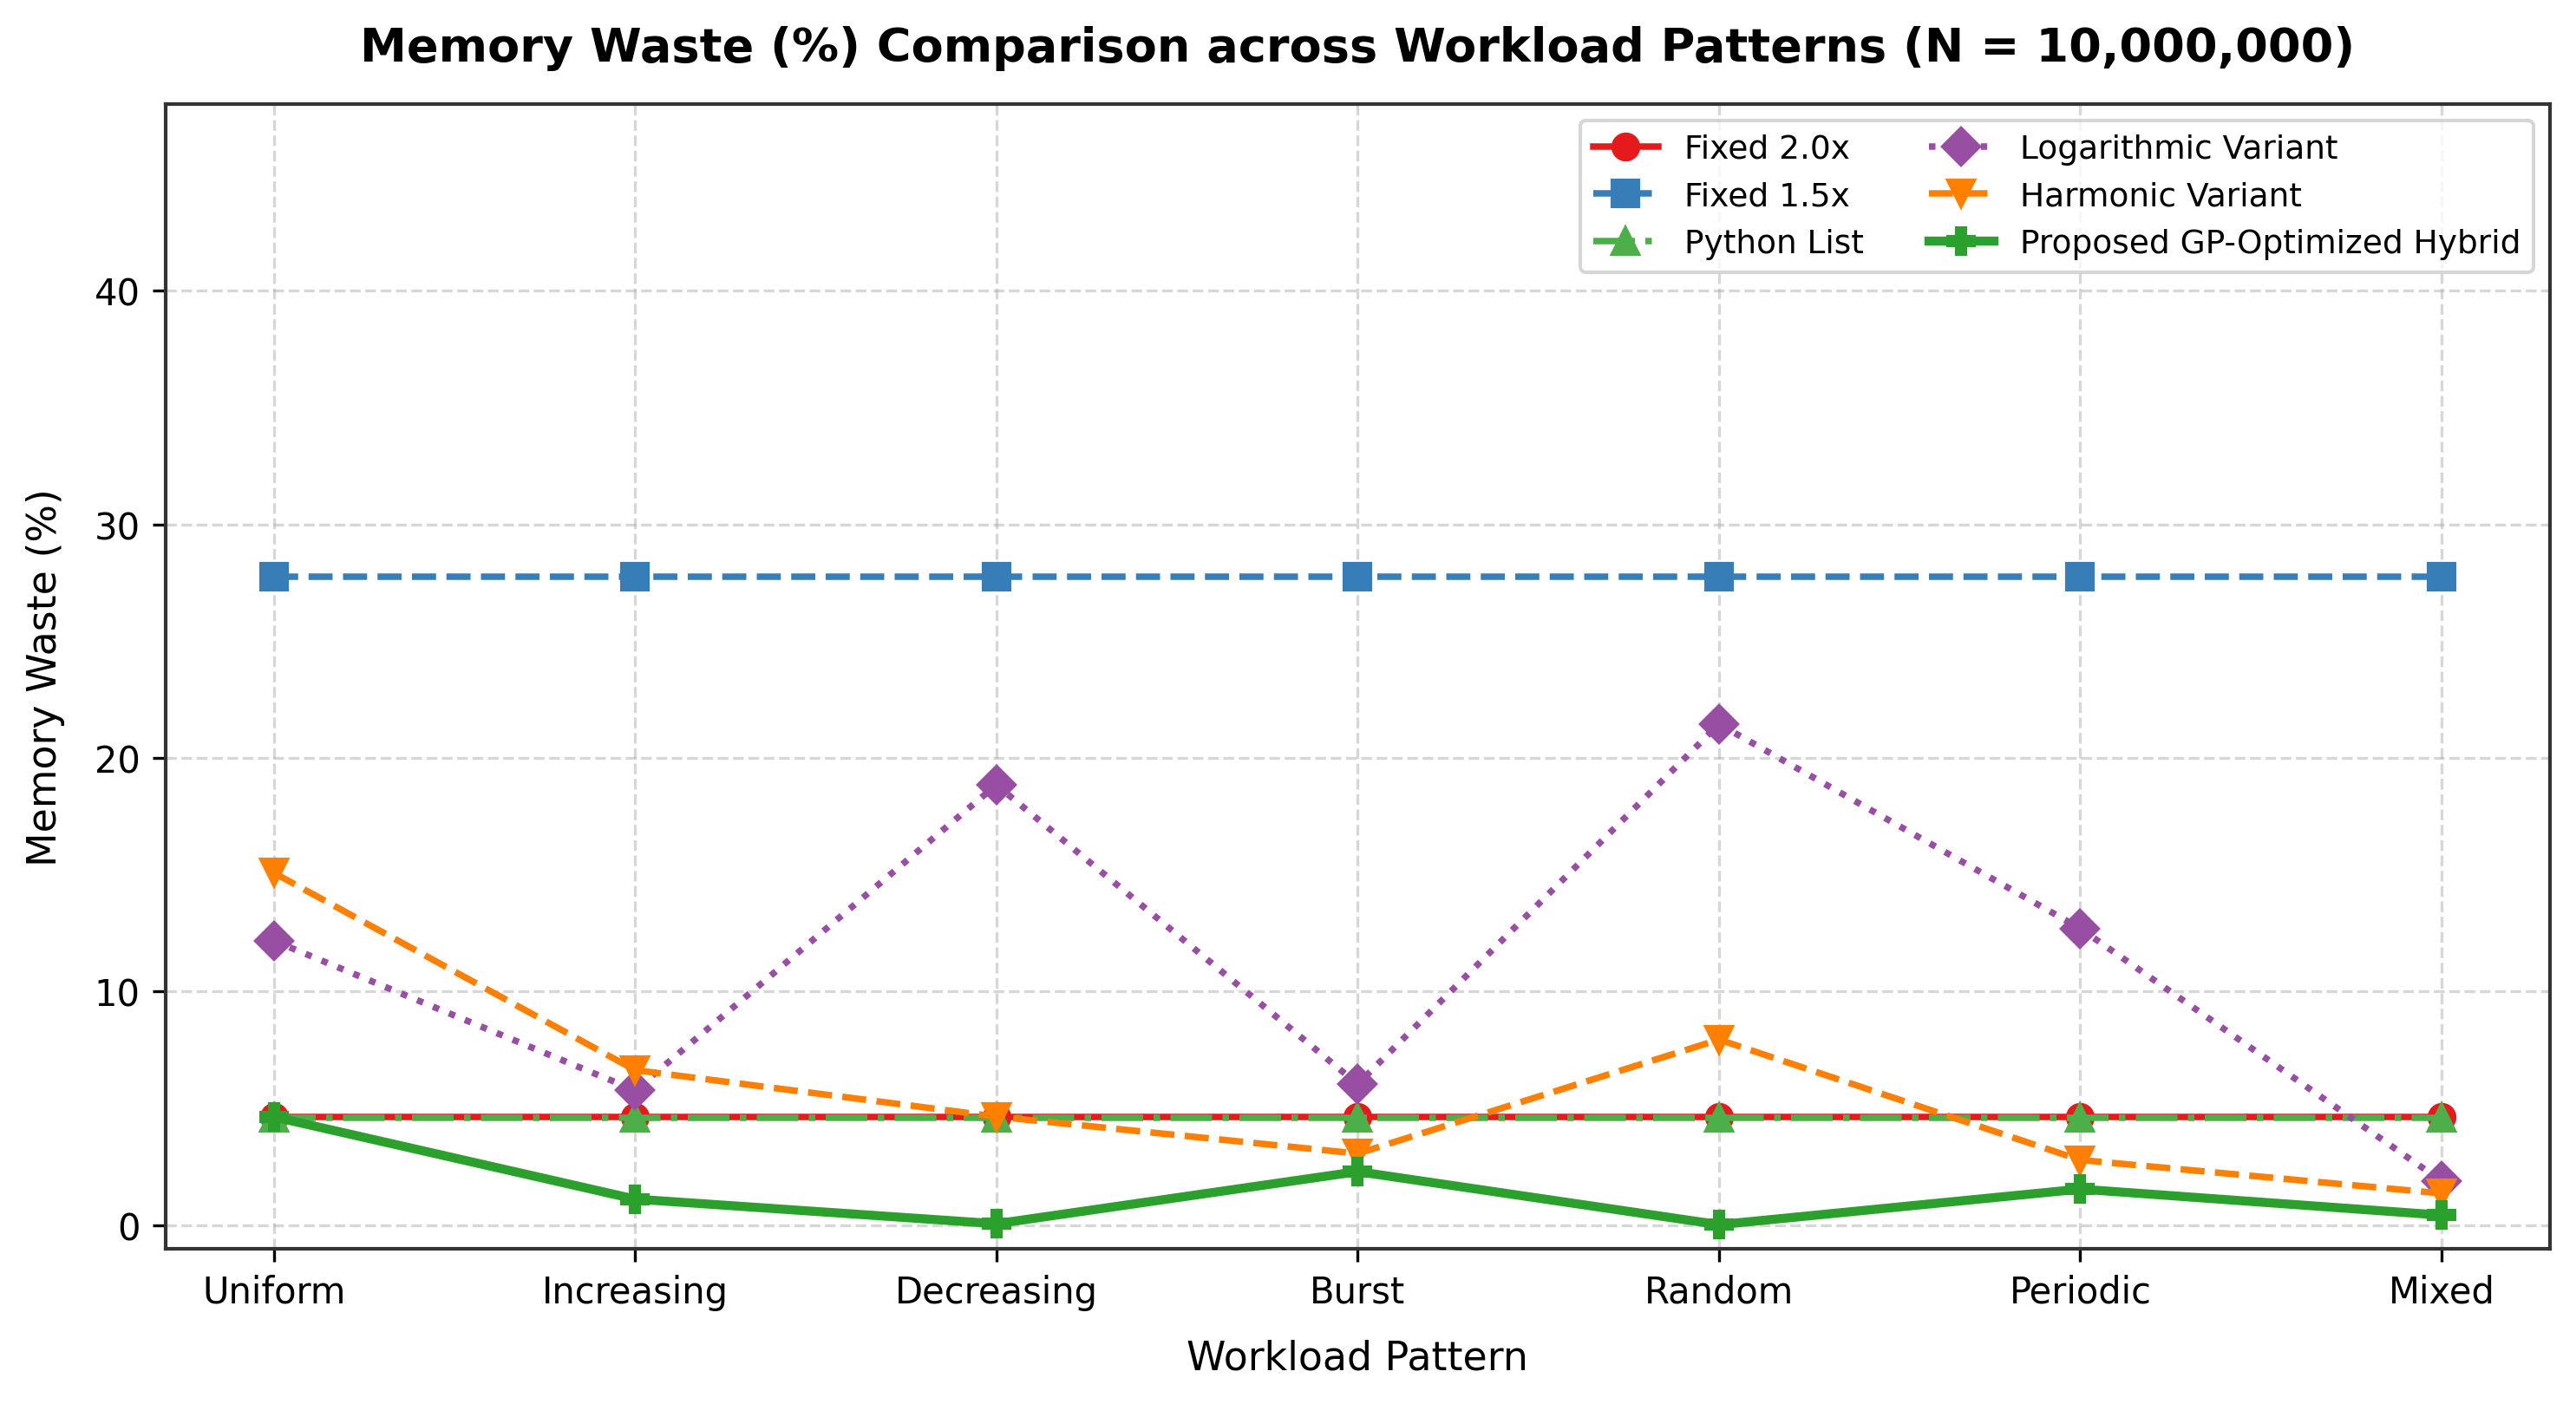
\includegraphics[width=0.95\linewidth]{fd_combined_patterns_line.png}}
\caption{Memory waste (\%) across seven workload patterns at $10^7$ insertions.}
\label{fig:memory_waste}
\end{figure} 

To isolate contribution of workload awareness, we compared the optimized model against an unmodulated baseline with $\lambda = 0$. Without velocity sensitivity ($\lambda = 0$), array cannot respond to sudden traffic surges, incurring additional reallocations during rapid ingestion. Calibrating $\lambda = 3.0944$ enables instantaneous responsiveness, dynamically expanding capacity during bursts while returning to conservative growth during steady phases.

\subsection{Scaling Behavior}
Fig.~\ref{fig:size_scaling} shows memory waste scaling across workload sizes from $10^4$ to $10^7$ elements.

\begin{figure}[htbp]
\centerline{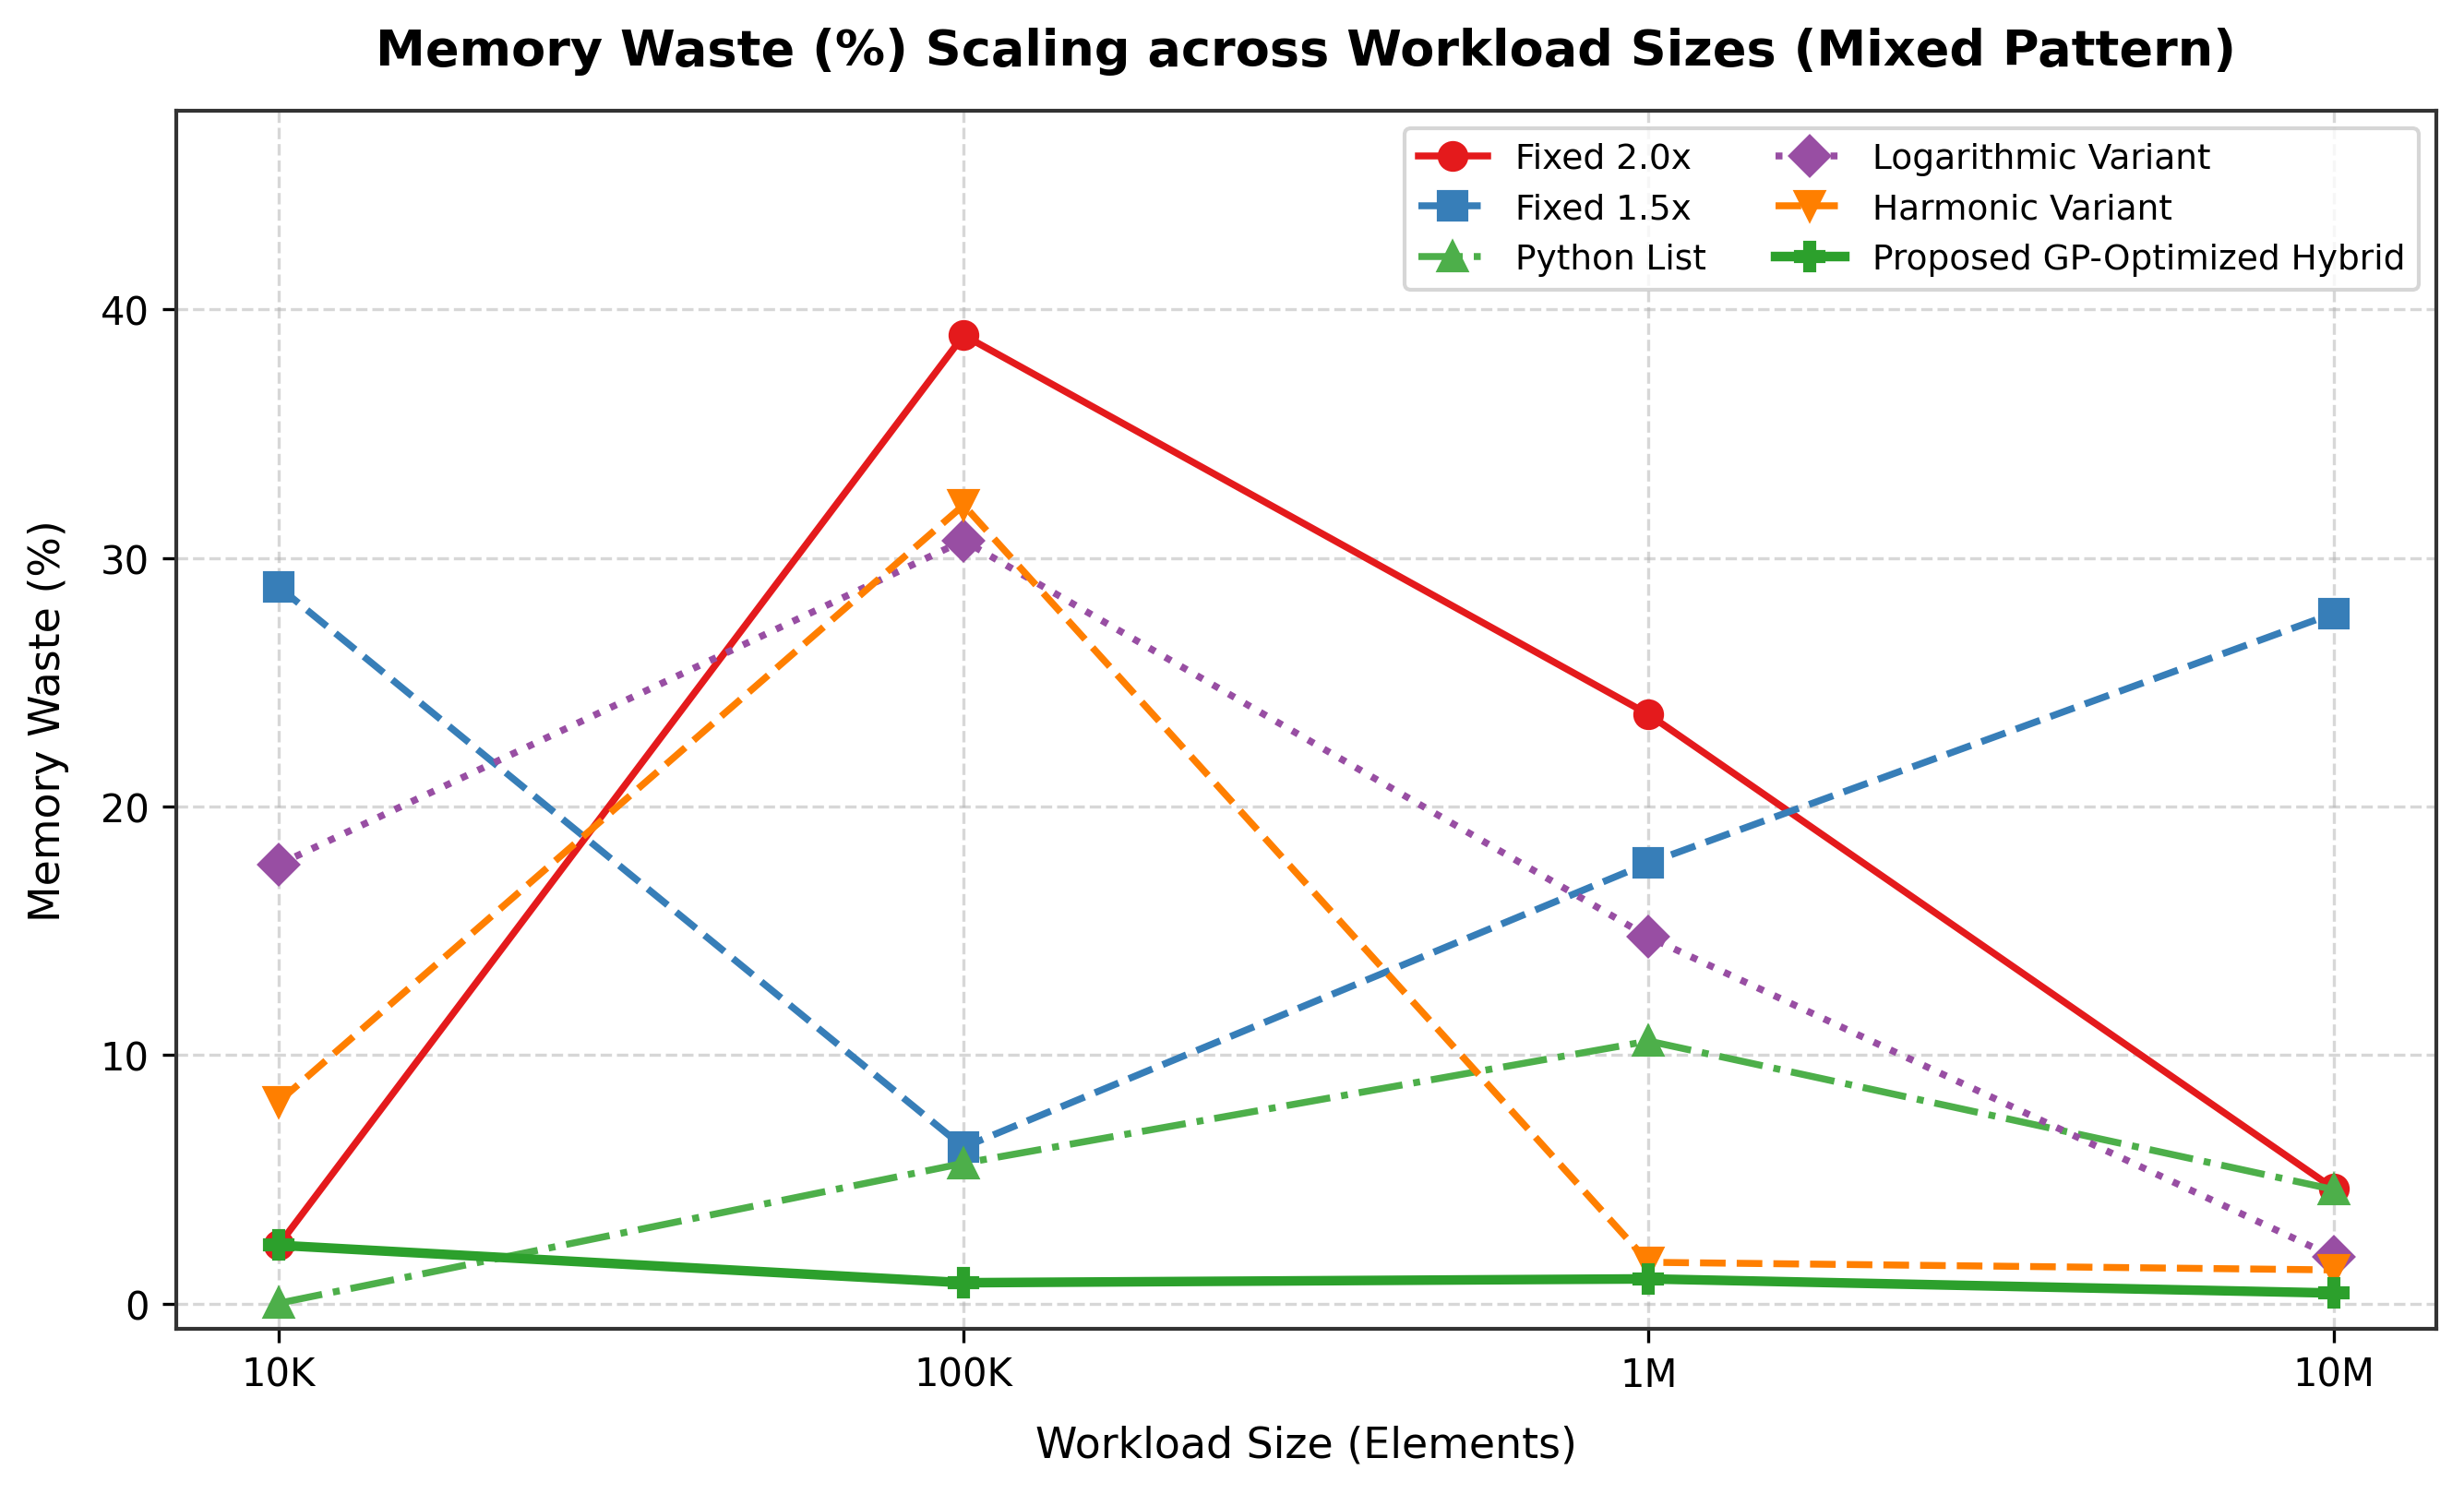
\includegraphics[width=0.95\linewidth]{fd_combined_workload_size_line.png}}
\caption{Memory waste (\%) vs.\ workload size under the mixed pattern.}
\label{fig:size_scaling}
\end{figure}

Scaling analysis indicates that memory waste exhibits non-monotonic fluctuation across workload scales due to discrete geometric reallocation boundaries. At intermediate scales (e.g., $10^6$ elements), capacity step alignment produces transient waste spikes (up to 8\% for the proposed method), but as scale expands to $10^7$, the proposed strategy converges to 0.42\% waste under mixed ingestion. Furthermore, while waste for Fixed $1.5\times$ fluctuates between 15\% and 30\% across scales, the proposed method maintains lower average spatial overhead. The simulated capacity, resize, and logical element-copy counts are independent of Python execution time, although their physical costs depend on the native implementation and allocator.

\section{Conclusion and Future Work}
This paper presents a workload-aware growth strategy for contiguous dynamic arrays that adjusts capacity expansion dynamically based on current capacity, resize iteration history, and real-time insertion velocity. By parameterizing a hybrid logarithmic--harmonic growth function using Gaussian-process Bayesian optimization, the proposed approach adapts to fluctuating ingestion rates while maintaining amortized $O(1)$ append complexity. Empirical evaluation across diverse workload patterns and scales demonstrates that adapting capacity growth directly to observed insertion intensity substantially restricts unused memory space without sacrificing reallocation performance or increasing element-copying overhead.

Future research will explore integrating the adaptive growth mechanism directly into native container runtimes, such as CPython (\texttt{listobject.c}) and C++ STL \texttt{std::vector}. Additionally, developing online Bayesian parameter updating will enable dynamic recalibration of optimization weights during live application execution. Finally, extending the workload-aware growth model to multidimensional dynamic arrays and lock-free concurrent sequences remains an important direction for future investigation.

\begin{thebibliography}{21}
\bibitem{cormen_algorithms}
T.~H. Cormen, C.~E. Leiserson, R.~L. Rivest, and C.~Stein, \emph{Introduction to Algorithms}, 4th~ed. Cambridge, MA, USA: MIT Press, 2022.

\bibitem{optimal_resizable}
A.~Brodnik, S.~Carlsson, E.~D. Demaine, J.~I. Munro, and R.~Sedgewick, ``Resizable Arrays in Optimal Time and Space,'' in \emph{Proc. 6th Int. Workshop Algorithms and Data Structures (WADS)}, 1999, pp. 37--48.

\bibitem{java_data_structures}
D.~E. Costa, A.~Andrzejak, J.~Seboek, and D.~Lo, ``Empirical Study of Usage and Performance of Java Collections,'' in \emph{Proc. 8th ACM/SPEC Int. Conf. Performance Engineering (ICPE)}, 2017, pp. 389--400.

\bibitem{python_list_impl}
Python Software Foundation, ``CPython List Object Implementation,'' CPython Source Code, GitHub Repository, \texttt{Objects/listobject.c}, v3.11.4, 2023.

\bibitem{time_space_complexity}
R.~E. Tarjan and U.~Zwick, ``Optimal Resizable Arrays,'' in \emph{Proc. 5th Symp. Simplicity in Algorithms (SOSA)}, 2023, pp. 1--10.

\bibitem{allocating_storage}
A.~L. Rosenberg, ``Allocating Storage for Extendible Arrays,'' \emph{Journal of the ACM}, vol. 21, no. 4, pp. 652--670, 1974.

\bibitem{managing_storage}
A.~L. Rosenberg, ``Managing Storage for Extendible Arrays,'' \emph{SIAM Journal on Computing}, vol. 4, no. 3, pp. 287--306, 1975.

\bibitem{logarithmic_arrays}
R.~R. Hoogerwoord, ``A Logarithmic Implementation of Flexible Arrays,'' in \emph{Proc. 2nd Int. Conf. Mathematics of Program Construction (MPC)}, 1992, pp. 191--207.

\bibitem{resizable_optimal_time_space}
P.~Bille, A.~R. Christiansen, M.~B. Ettienne, and I.~L. G{\o}rtz, ``Fast Dynamic Arrays,'' in \emph{Proc. 25th Annual European Symposium on Algorithms (ESA)}, 2017, pp. 16:1--16:13.

\bibitem{fast_array}
J.~Katajainen, ``Worst-case-efficient Dynamic Arrays in Practice,'' in \emph{Proc. 15th Int. Symposium on Experimental Algorithms (SEA)}, 2016, pp. 167--183.

\bibitem{z_rays}
J.~B. Sartor, S.~M. Blackburn, D.~Frampton, M.~Hirzel, and K.~S. McKinley, ``Z-rays: Divide Arrays and Conquer Speed and Flexibility,'' in \emph{Proc. 31st ACM SIGPLAN Conf. Programming Language Design and Implementation (PLDI)}, 2010, pp. 406--417.

\bibitem{lock_free_vector}
D.~Dechev, P.~Pirkelbauer, and B.~Stroustrup, ``Lock-Free Dynamically Resizable Arrays,'' in \emph{Proc. 10th Int. Conf. Principles of Distributed Systems (OPODIS)}, 2006, pp. 142--156.

\bibitem{persistent_arrays}
P.~F. Dietz, ``Fully Persistent Arrays,'' in \emph{Proc. 1st Workshop on Algorithms and Data Structures (WADS)}, 1989, pp. 67--74.

\bibitem{dynamic_storage_allocation}
P.~R. Wilson, M.~S. Johnstone, M.~Neely, and D.~Boles, ``Dynamic Storage Allocation: A Survey and Critical Review,'' in \emph{Proc. 1st Int. Workshop on Memory Management (IWMM)}, 1995, pp. 1--116.

\bibitem{reconsidering_custom_allocation}
E.~D. Berger, B.~G. Zorn, and K.~S. McKinley, ``Reconsidering Custom Memory Allocation,'' in \emph{Proc. 17th ACM SIGPLAN Conf. Object-Oriented Programming, Systems, Languages, and Applications (OOPSLA)}, 2002, pp. 1--12.

\bibitem{hoard_allocator}
E.~D. Berger, K.~S. McKinley, R.~D. Blumofe, and P.~R. Wilson, ``Hoard: A Scalable Memory Allocator for Multithreaded Applications,'' in \emph{Proc. 9th Int. Conf. Architectural Support for Programming Languages and Operating Systems (ASPLOS)}, 2000, pp. 117--128.

\bibitem{frigo_cache_oblivious}
M.~Frigo, C.~E. Leiserson, H.~Prokop, and S.~Ramachandran, ``Cache-Oblivious Algorithms,'' in \emph{Proc. 40th Annual Symposium on Foundations of Computer Science (FOCS)}, 1999, pp. 285--297.

\bibitem{practical_bayesian_opt}
J.~Snoek, H.~Larochelle, and R.~P. Adams, ``Practical Bayesian Optimization of Machine Learning Algorithms,'' in \emph{Proc. 25th Int. Conf. Neural Information Processing Systems (NIPS)}, 2012, pp. 2951--2959.

\bibitem{bayesian_opt_review}
B.~Shahriari, K.~Swersky, Z.~Wang, R.~P. Adams, and N.~de Freitas, ``Taking the Human Out of the Loop: A Review of Bayesian Optimization,'' \emph{Proceedings of the IEEE}, vol. 104, no. 1, pp. 148--175, 2016.

\bibitem{jones_ego}
D.~R. Jones, M.~Schonlau, and W.~J. Welch, ``Efficient Global Optimization of Expensive Black-Box Functions,'' \emph{Journal of Global Optimization}, vol. 13, no. 4, pp. 455--492, 1998.

\bibitem{scikit_optimize}
T.~Head, M.~Kumar, H.~Nahrstaedt, G.~Louppe, and I.~Shcherbatyi, ``scikit-optimize: Sequential model-based optimization in Python,'' \emph{Zenodo}, v0.5.2, DOI: 10.5281/zenodo.1208477, 2018.
\end{thebibliography}

\end{document}
